\documentclass[12pt]{article}

\author{Alok Kumar}
\title{Titanc}

\usepackage{Sweave}
\begin{document}
\input{Example-concordance}

  \maketitle

\section*{Data Collection :}
There is two type of data set 


\begin{Schunk}
\begin{Sinput}
> train.df = read.csv("Data/train.csv", 
+                     stringsAsFactors = FALSE, 
+                     na.strings = c(""), 
+                     header = T)  
> test.df = read.csv("Data/test.csv", 
+                    stringsAsFactors = FALSE, 
+                    na.strings = c(""), 
+                    header = T)
\end{Sinput}
\end{Schunk}

\section*{Exploring Data:}

The trained dataset contains 891 observations and 12 features (Variable), and the tested dataset contains 418 observations.

\begin{Schunk}
\begin{Sinput}
> str(train.df)
\end{Sinput}
\begin{Soutput}
'data.frame':	891 obs. of  12 variables:
 $ PassengerId: int  1 2 3 4 5 6 7 8 9 10 ...
 $ Survived   : int  0 1 1 1 0 0 0 0 1 1 ...
 $ Pclass     : int  3 1 3 1 3 3 1 3 3 2 ...
 $ Name       : chr  "Braund, Mr. Owen Harris" "Cumings, Mrs. John Bradley (Florence Briggs Thayer)" "Heikkinen, Miss. Laina" "Futrelle, Mrs. Jacques Heath (Lily May Peel)" ...
 $ Sex        : chr  "male" "female" "female" "female" ...
 $ Age        : num  22 38 26 35 35 NA 54 2 27 14 ...
 $ SibSp      : int  1 1 0 1 0 0 0 3 0 1 ...
 $ Parch      : int  0 0 0 0 0 0 0 1 2 0 ...
 $ Ticket     : chr  "A/5 21171" "PC 17599" "STON/O2. 3101282" "113803" ...
 $ Fare       : num  7.25 71.28 7.92 53.1 8.05 ...
 $ Cabin      : chr  NA "C85" NA "C123" ...
 $ Embarked   : chr  "S" "C" "S" "S" ...
\end{Soutput}
\end{Schunk}

\section*{Preparion Data:}


\subsection*{Missing Data Analysis }
We have to analyse is there any missing data.
\begin{Schunk}
\begin{Sinput}
> sapply(train.df, function(x) sum(is.na(x)))
\end{Sinput}
\begin{Soutput}
PassengerId    Survived      Pclass        Name         Sex         Age 
          0           0           0           0           0         177 
      SibSp       Parch      Ticket        Fare       Cabin    Embarked 
          0           0           0           0         687           2 
\end{Soutput}
\end{Schunk}

Age and cabin need to handle. Lets check what fraction of data is missing in both.

\subsubsection*{Cabin}
\begin{Schunk}
\begin{Sinput}
> train.df['CabinMissing'] =  sapply(train.df$Cabin, 
+                                    function(x) 
+                                      ifelse(is.na(x),
+                                         "Missing","Avalable")
+                                    )
> barplot(table(factor(train.df$CabinMissing)), 
+         main = "Train Cabin Missing vs Avalable Data")
> 
\end{Sinput}
\end{Schunk}
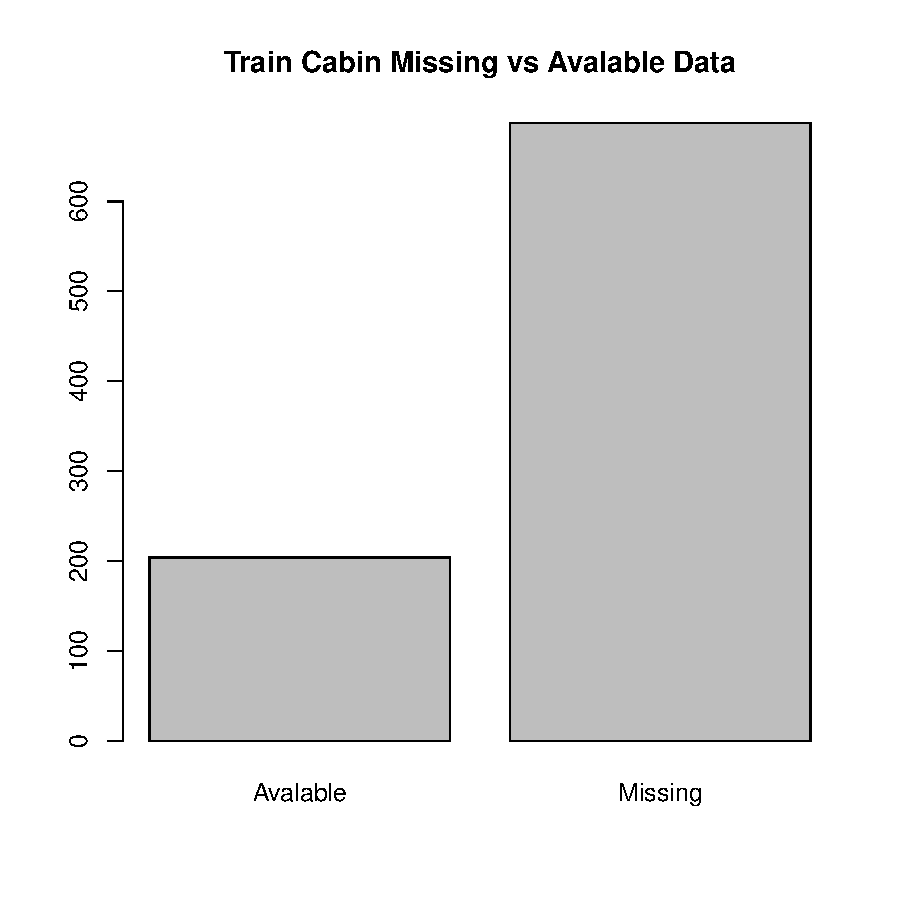
\includegraphics{Example-004}

\subsubsection*{Age}
\begin{Schunk}
\begin{Sinput}
> train.df['AgeMissing'] =  sapply(train.df$Age, 
+                                  function(x) 
+                                   ifelse(is.na(x),
+                                     "Missing","Avalable")
+                                  )
> barplot(table(factor(train.df$AgeMissing)), 
+         main = "Train Age Missing vs Avalable")
\end{Sinput}
\end{Schunk}
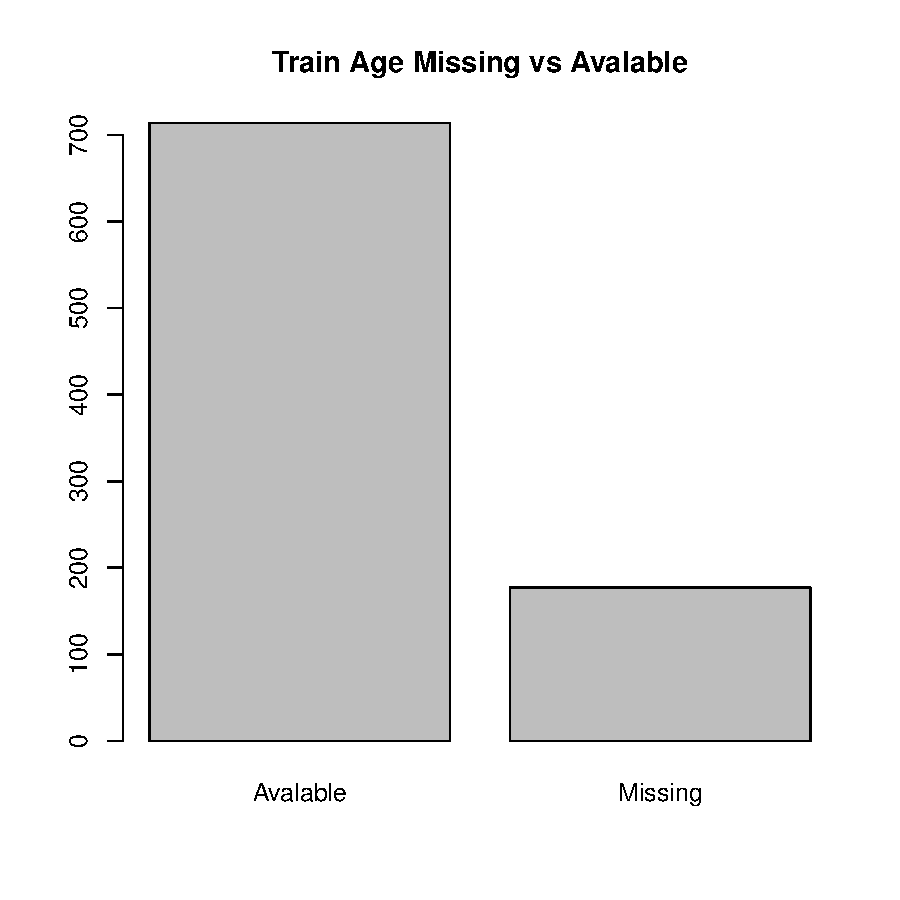
\includegraphics{Example-005}

Since cabin have many missing data we can remove this feather from out data set.

\begin{Schunk}
\begin{Sinput}
> train.df  = subset(train.df, select = c(2,3,5,6,7,8,10,12))
> 
\end{Sinput}
\end{Schunk}

To handle missing value of Age we can apply one of these method.
\begin{itemize}
  \item Throw out any data with missing values
  \item Assign the average value
  \item Use a regression or another simple model to predict the values of missing variables
\end{itemize}

For checking weather we can use regression or not lets check correlation in predicter. 

\begin{Schunk}
\begin{Sinput}
> corr = na.omit(train.df)
> cormat <- round(cor(corr[, c('Age','Fare')]),2)
> cormat
\end{Sinput}
\begin{Soutput}
      Age Fare
Age  1.00 0.09
Fare 0.09 1.00
\end{Soutput}
\begin{Sinput}
> cormat <- round(cor(corr[, c('Age','Parch')]),2)
> cormat
\end{Sinput}
\begin{Soutput}
        Age Parch
Age    1.00 -0.19
Parch -0.19  1.00
\end{Soutput}
\begin{Sinput}
> cormat <- round(cor(corr[, c('Age','Sex')]),2)